\section{Physical model and free-energy functional}
We study a one-dimensional altermagnetic superconductor in the Nambu basis
$\Psi_k=(c_{k+q/2,\uparrow},c_{k+q/2,\downarrow},c^\dagger_{-k+q/2,\uparrow},c^\dagger_{-k+q/2,\downarrow})^T$ with
\begin{equation}
H_{\rm BdG}(k)=\begin{pmatrix}h(k+q/2)-\mu&\Delta_q\\ \Delta_q^*&-\sigma_y h^T(-k+q/2)\sigma_y+\mu\end{pmatrix},
\end{equation}
where $h(k)=t\cos k+(0,\lambda_y\sin k,\lambda_z\sin k+J_A\cos k)\cdot\boldsymbol\sigma$.
The implementation evaluates the normal-referenced discrete free energy
\begin{equation}
F(\Delta,q)=\frac{1}{2N_k}\sum_{k,n}E_n(k;\Delta,q)f[E_n/(k_BT)]+\frac{\Delta^2}{U}-\frac{1}{2N_k}\sum_{k,n}E_n(k;0,q)f[E_n(k;0,q)/(k_BT)],
\end{equation}
with $f(z)=1/(e^z+1)$ in a numerically stable sigmoid form.  The final term defines the normal reference.  All energies are reported in units of $t$.

\begin{table}[h]\caption{Physical and numerical parameters.}\label{tab:s1}\centering\small
\begin{tabular}{lll}\toprule Quantity & Value & Role\\\midrule
$t$ & 1 & energy unit\\ $\lambda_y,\lambda_z$ & 0.6, 0.6 & spin--orbit couplings\\ $\mu$ & 0.55 & 2D chemical potential\\ $U$ & 1.6 & pairing interaction\\ $\omega_D$ & 10 & momentum mask cutoff\\ $N_k$ & 800 & Brillouin-zone grid\\ coarse $\Delta$ grid & $[0,0.6]$, 400 points & thermodynamic scan\\ initial $q$ grid & $[-1,0.5]$, 400 points & momentum scan\\ $\Delta_\epsilon,q_\epsilon$ & $10^{-3},10^{-2}$ & phase assignment\\\bottomrule\end{tabular}\end{table}

\section{Exact BdG oracle}
\paragraph{Algorithm S1: Exact thermodynamic and topology oracle.}
For each requested coordinate: (1) construct the BdG spectrum on the coarse $(\Delta,q)$ grid; (2) form the normal-referenced free energy; (3) detect global, near-degenerate, and edge-risk minima; (4) expand the $q$ window directionally when the low-energy structure is not enclosed, up to three expansions; (5) refine selected local basins using at least 800 $q$ points and 600 $\Delta$ points in the adaptive-box path; (6) compare near-zero-$\Delta$ states with a strictly positive-$\Delta$ scan; (7) assign the thermodynamic phase and a separate numerical status; (8) return flagged points for retention or rerun rather than silently treating them as reliable; and (9) if the state is reliable, gapped, and FFLO, evaluate the full-zone gap and Pfaffians.  Duplicate coordinates are reconciled by the configured four-decimal key before append.

\section{Reliability-state hierarchy}
Accepted/reliable points have an enclosed minimum and a resolved normal-state comparison. Boundary-delicate points lie within the adopted finite energy or order-parameter resolution. A $q$-window-unresolved point retains low-energy structure at the scanned edge after allowed expansion; a near-zero-$\Delta$-unresolved point lacks a resolved condensation-energy sign. Rerun-required records remain outside the clean physical training view. Topology-inapplicable includes all non-FFLO or numerically unreliable states, while gap-unresolved states do not receive a $\mathbb Z_2$ label. Phase identity, training eligibility, rerun status, and topology applicability are separate fields.
\begin{figure}[h]\centering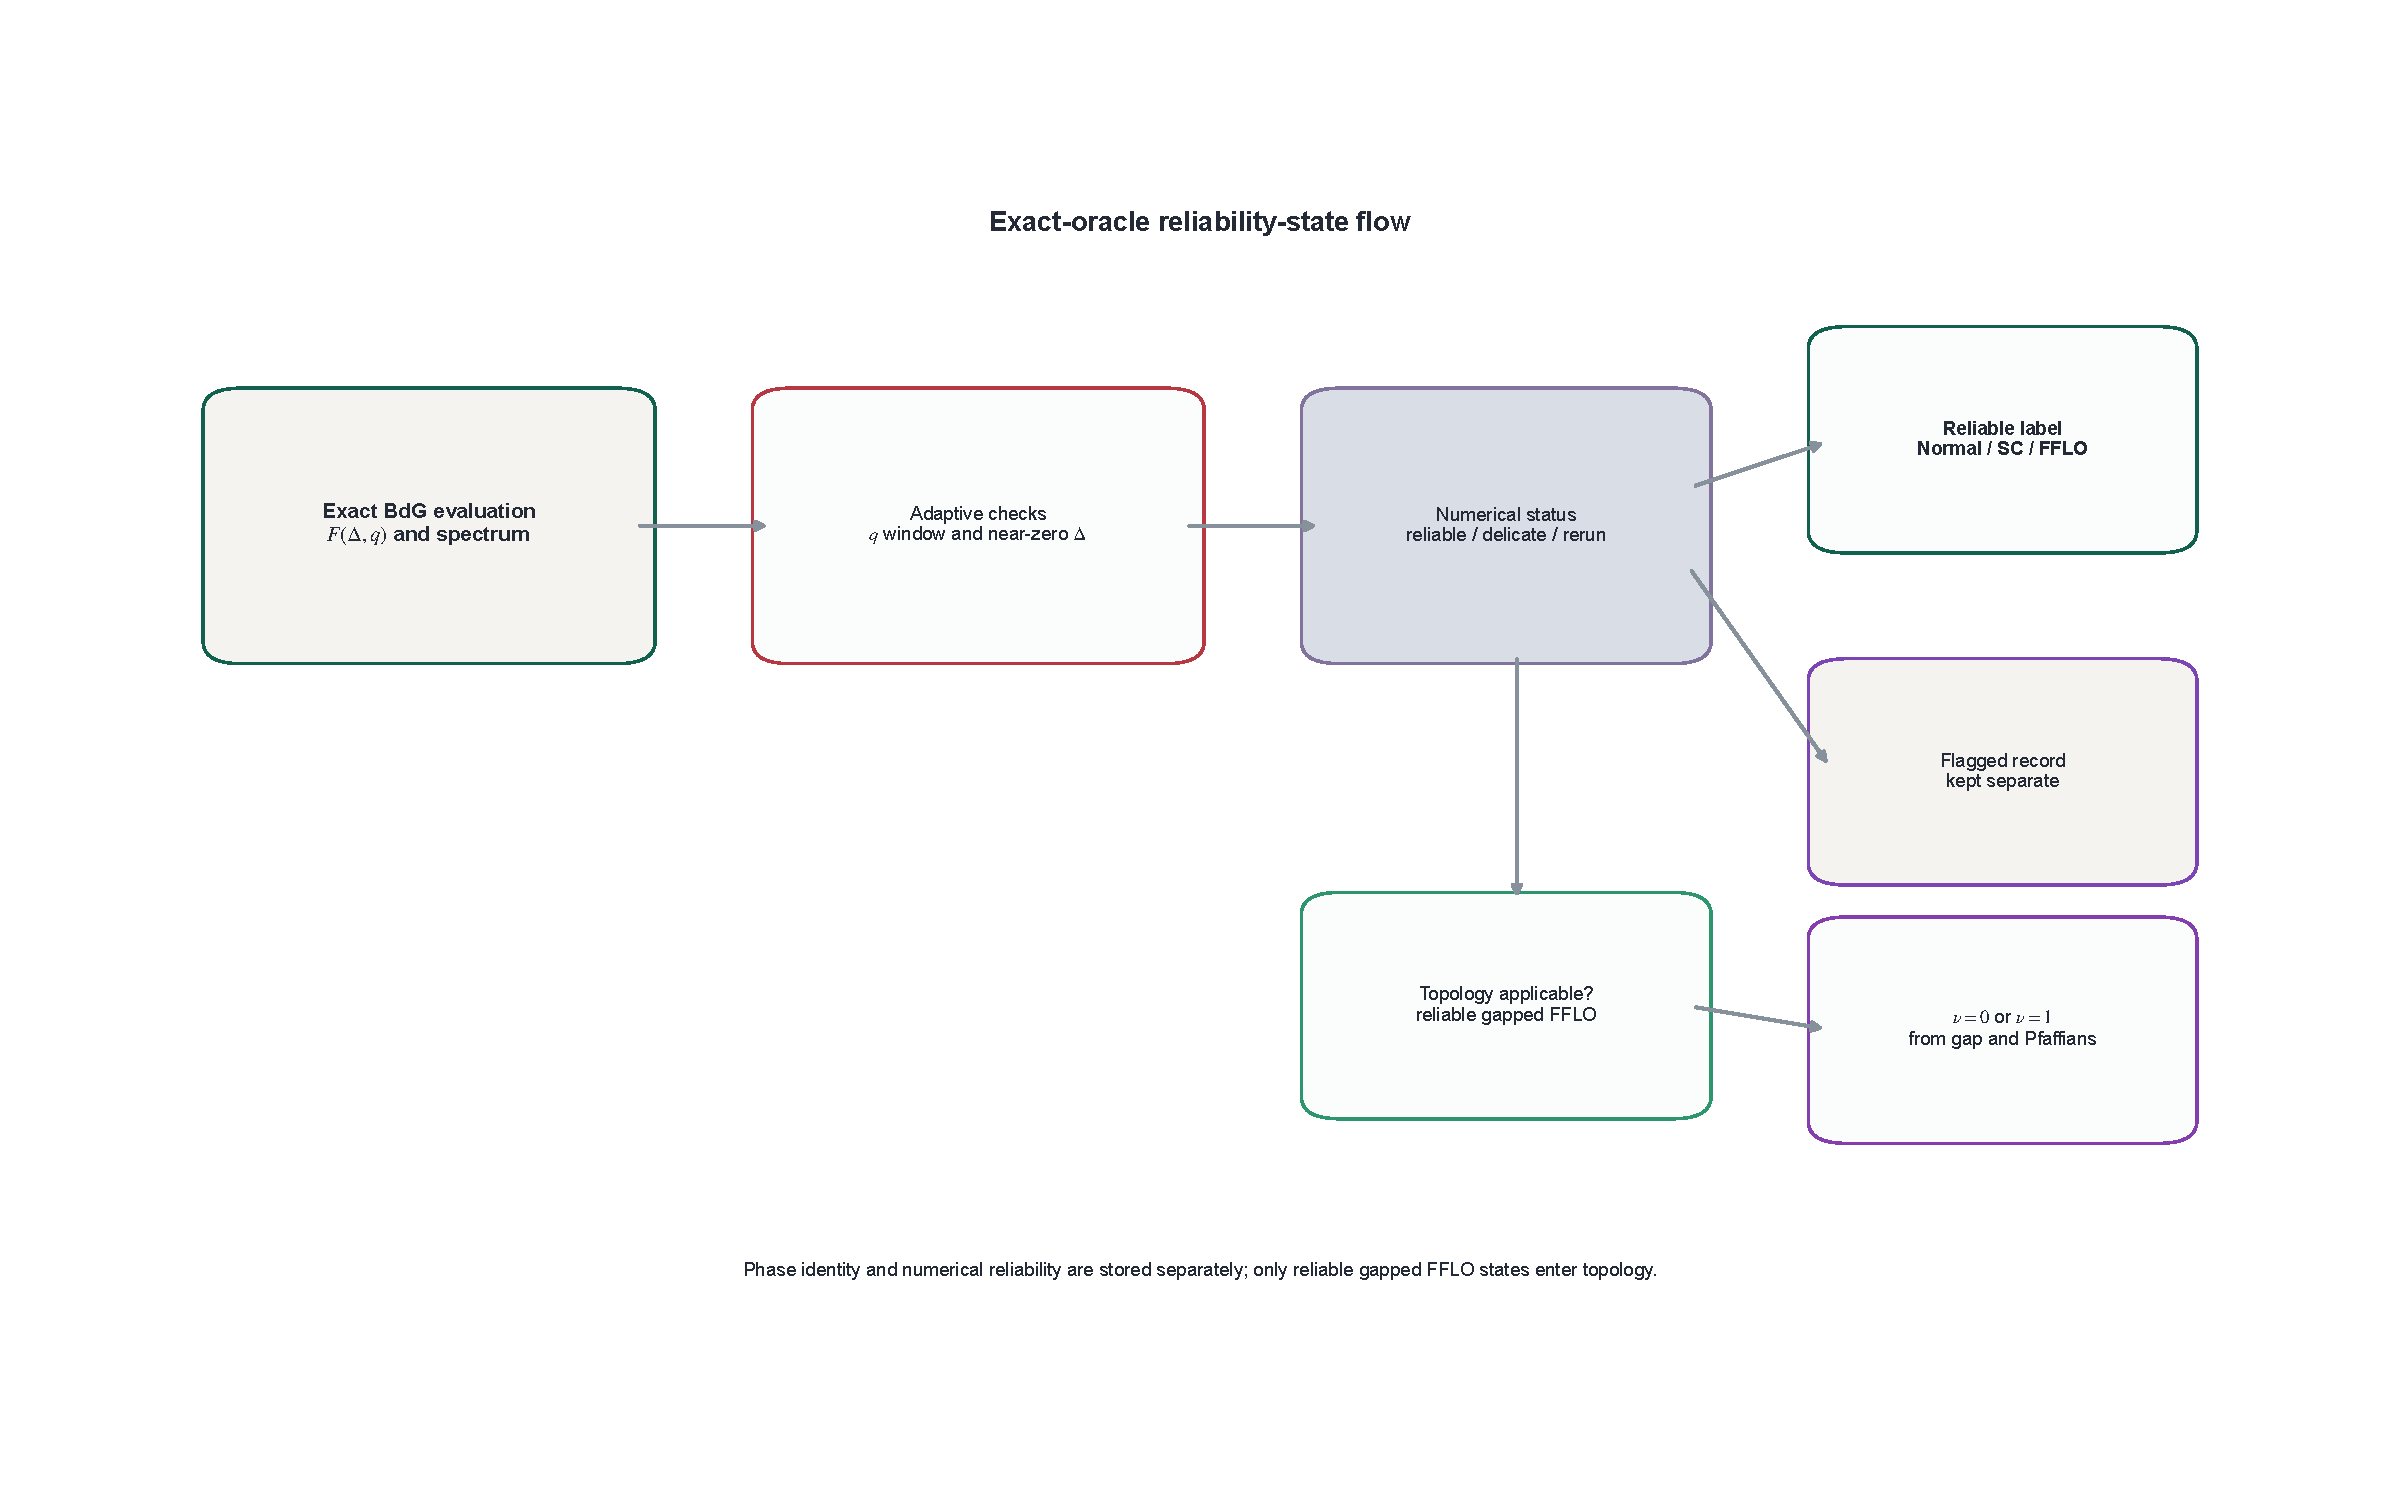
\includegraphics[width=\columnwidth]{figures/S1_reliability_flow.pdf}\caption{Exact-oracle reliability-state flow.  Numerical status is separate from phase identity, and topology is restricted to reliable gapped FFLO states.}\end{figure}

\section{Complete active-learning loop}
\paragraph{Algorithm S2: Reliability-aware active learning.}
(1) Draw a 512-point random-grid cold start from the full candidate domain. (2) Construct the training-eligible exact view and a phase-stratified 85/15 training/validation split. (3) Train independent regression and classification ensembles from scratch with deterministic member seeds. (4) predict all unseen candidate locations; (5) compute acquisition components and apply the candidate mask, exact-coordinate exclusion, active-pool rule, and observation repulsion; (6) construct a stochastic microbatch with within-batch repulsion; (7) write restartable point shards; (8) run the exact BdG oracle; (9) merge returned shards and separate reliable, delicate, and rerun records; (10) append eligible unique observations; and (11) recompute fixed-grid diagnostics and continue until an operational stop or budget limit.  Checkpoints include the dataset, selection tables, run configuration, monitor predictions, stop history, and shard metadata. Stage III adds topology applicability and spectral acquisition components; Stage IV replaces the Cartesian 2D pool by a three-coordinate candidate construction but retains exact-label authority.

\section{Surrogate architecture and training}
The implementation uses separate PyTorch ensembles for regression and phase classification, not a Gaussian process or tree model. Each of five members is an MLP with two 64-unit hidden layers and ReLU activations. Inputs are standardized by the training mean and standard deviation. Regression targets $(\Delta,q,\eta,I_c^+,I_c^-)$ are also standardized; the regression loss is mean-squared error. The classifier uses cross entropy on Normal, uniform-SC, and FFLO labels. Adam uses learning rate $10^{-3}$ and weight decay $10^{-5}$, batch size 512, and 240 epochs for both tasks. Members use seeds $42+1000+i$ and $42+2000+i$ for regression and classification. Models are retrained from scratch at each scheduling step; no early-stopping rule is implemented in these model classes. Regression uncertainty is the member standard deviation; phase probabilities are averaged over members and converted to entropy and margin scores.
\begin{table}[h]\caption{Surrogate and training hyperparameters.}\centering\small\begin{tabular}{ll}\toprule Item&Value\\\midrule ensemble size&5 per task\\ hidden layers&2 $\times$ 64, ReLU\\ validation fraction&0.15, phase stratified\\ optimizer&Adam\\ learning rate / weight decay&$10^{-3}/10^{-5}$\\ epochs / batch size&240 / 512\\ regression loss&MSE\\ classification loss&cross entropy\\ uncertainty&member dispersion / averaged probabilities\\\bottomrule\end{tabular}\end{table}
\begin{figure}[h]\centering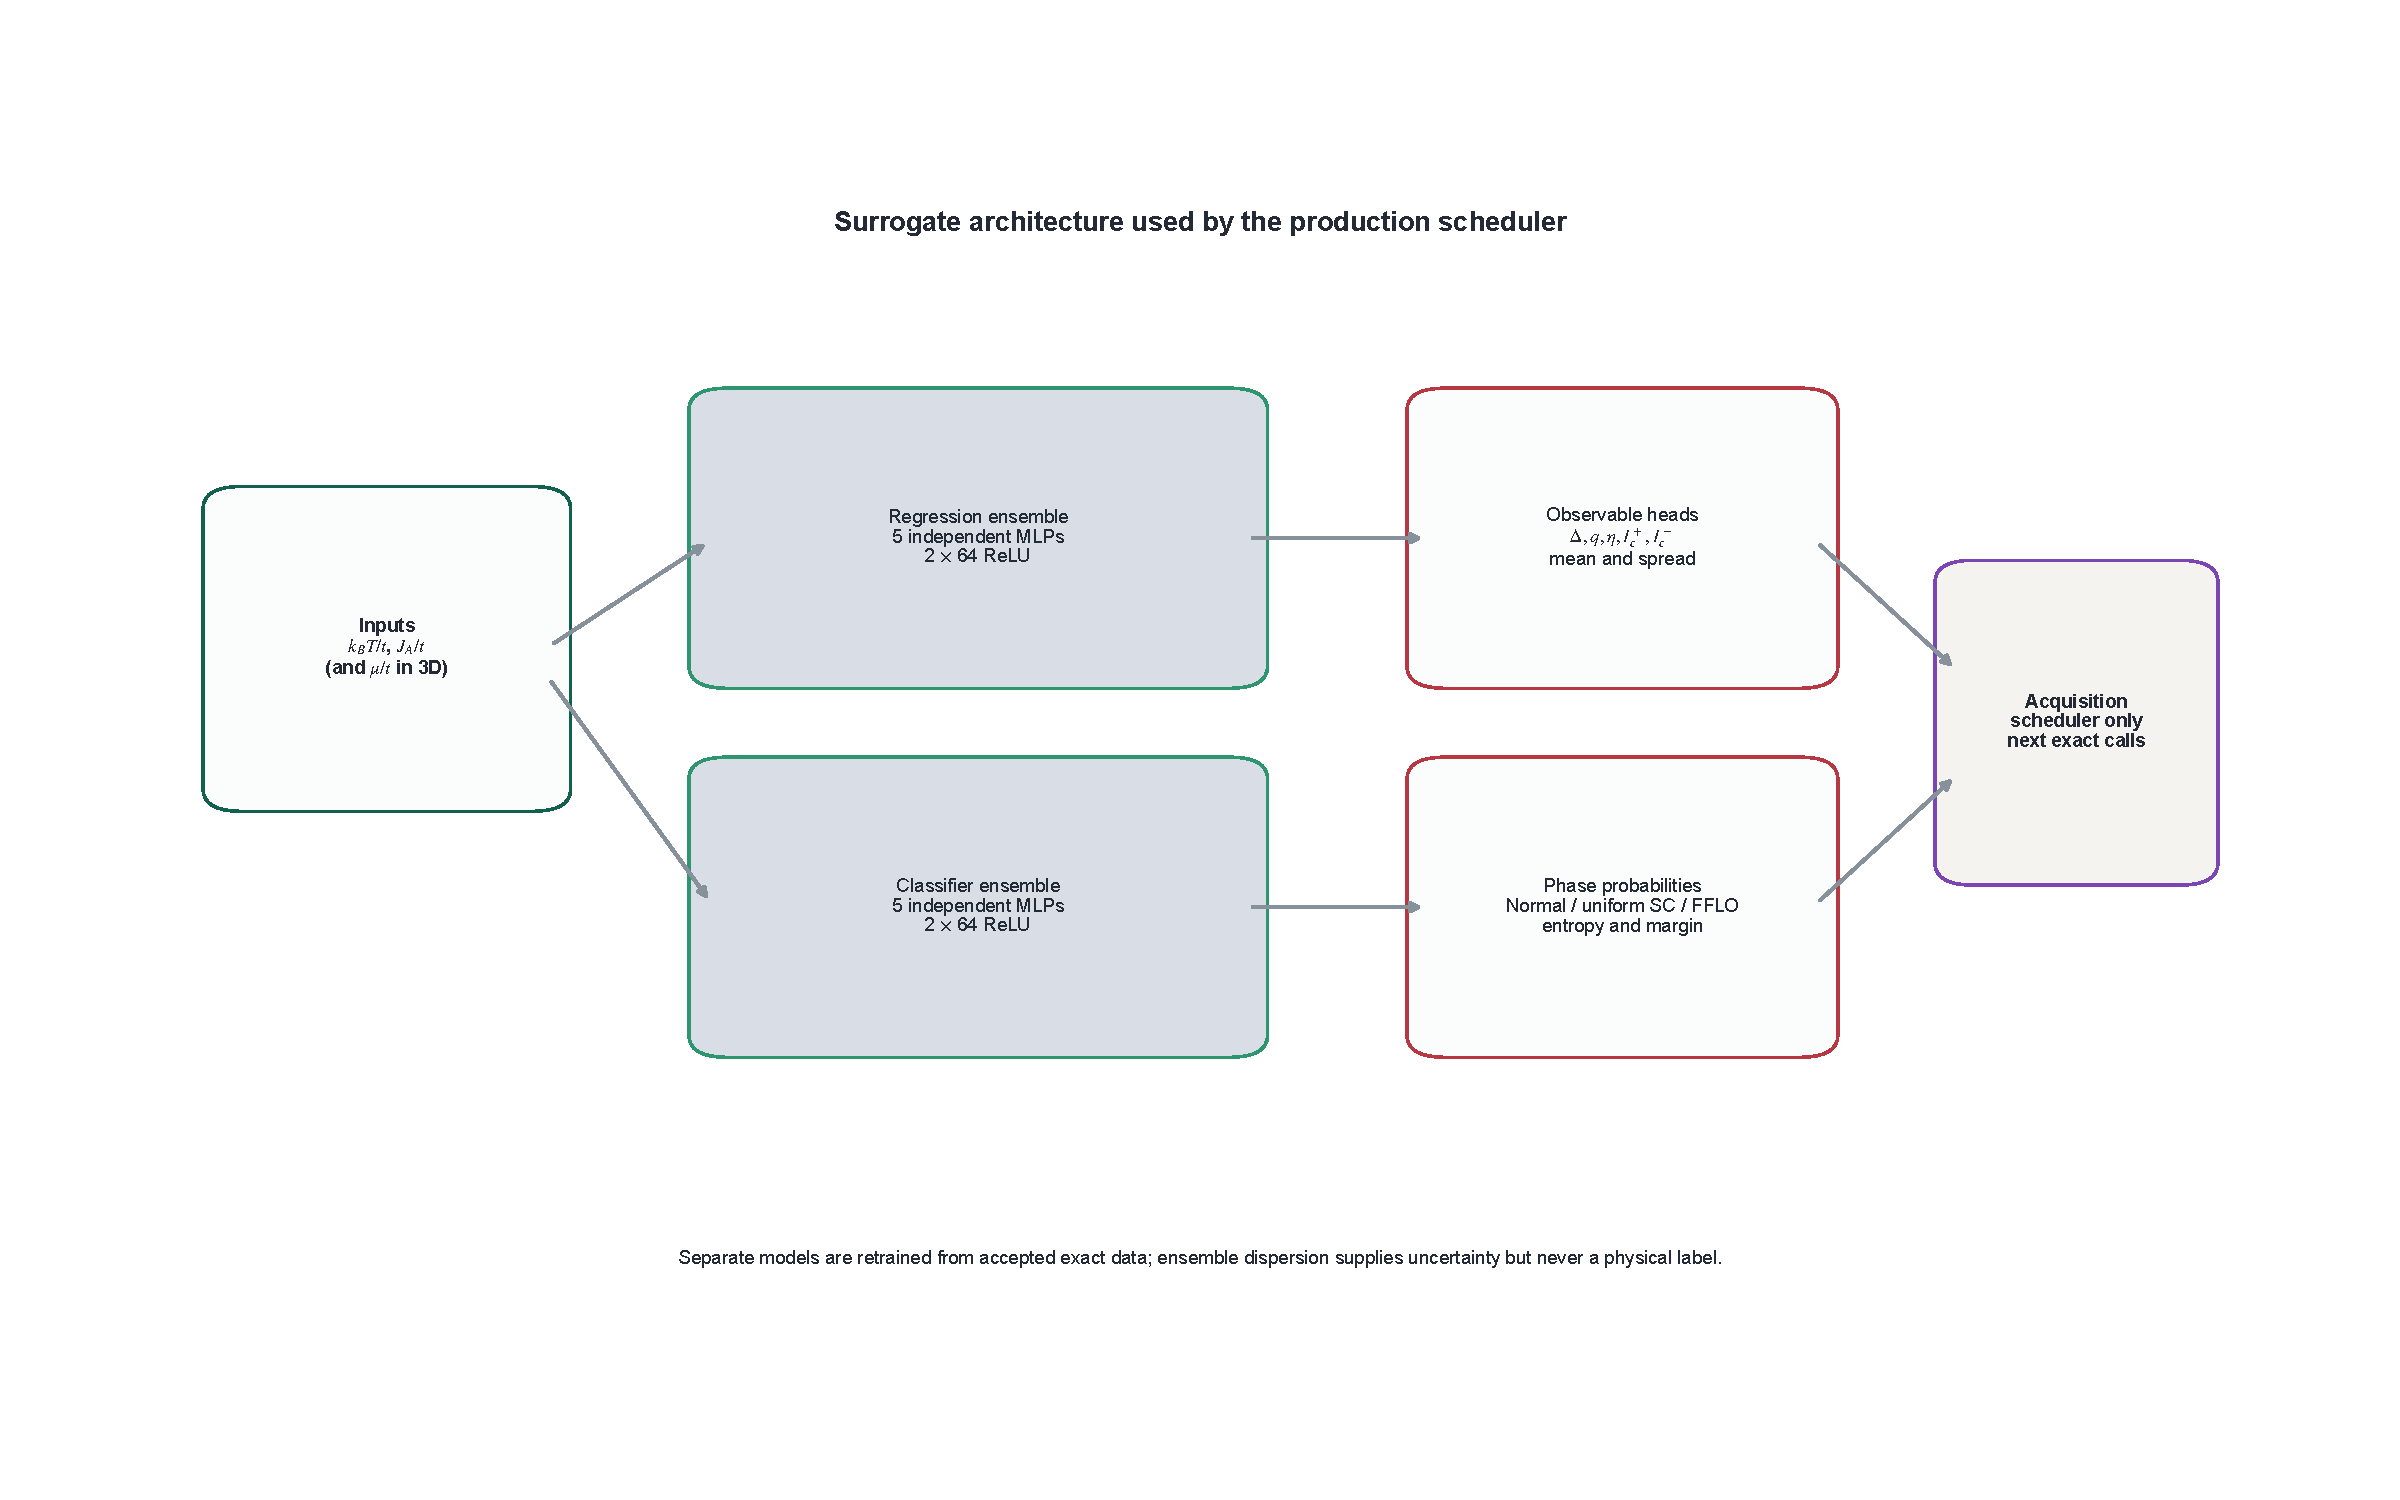
\includegraphics[width=\columnwidth]{figures/S2_surrogate_architecture.pdf}\caption{Production surrogate architecture.  The regression and classification ensembles supply scheduling scores, not physical labels.}\end{figure}

\section{Acquisition function and microbatch selection}
Let $U_{\rm cls}=0.4H+0.6\exp[-m/0.2]$, where $H$ is normalized phase entropy and $m$ is the largest-probability margin. Let $U_{\rm reg}=(U_\Delta+U_q)/2$, $B_{NS}=\exp[-|\hat\Delta-\Delta_\epsilon|/0.04]\,4P_NP_{SC}$, $B_{UF}=P_{SC}\exp[-||\hat q|-q_\epsilon|/0.04]$, and $G=(G_\Delta+G_q)/2$.  The production profile is
\begin{equation} A_{\rm phase}=U_{\rm cls}+0.6U_{\rm reg}+B_{NS}+0.9B_{UF}+0.5G,\qquad A_0=A_{\rm phase}+0.4E_q+w_{\rm ext}E_{\rm ext},\end{equation}
where $E_q$ flags predicted $q$-edge risk and $E_{\rm ext}$ combines extrapolation with uncertainty. $w_{\rm ext}$ decreases piecewise from 0.15 to 0.08 and 0.03 at iterations 10 and 30. High-confidence interiors receive a soft penalty; the active pool is set by the larger of a scheduled quantile and $0.7p_{95}(A_0)$.  Observation repulsion uses length 0.02 and floor 0.5. During greedy stochastic construction, batch repulsion uses length 0.03 and floor 0.01, yielding $A_{\rm select}=A_0R_{\rm obs}R_{\rm batch}$ and sampling probability proportional to $A_{\rm select}^\gamma$, with $\gamma=1.5,2.5,4.0$ across the same schedule. Existing exact coordinates are excluded before selection.
\paragraph{Algorithm S3: Repelled microbatch construction.} Build the active pool from $A_0$ after masks and interior penalties; multiply by observation repulsion; sample one coordinate using the scheduled power; update $R_{\rm batch}$ around that coordinate; repeat until the requested batch is reached or the high-information pool is exhausted.
\begin{table*}[t]\caption{Production acquisition components.}\centering\small\begin{tabular}{llll}\toprule Component&Definition&Normalization or weight&Role\\\midrule phase entropy/margin&$U_{\rm cls}$&0.4/0.6 mixture&classification ambiguity\\ regression spread&$U_{\rm reg}$&min--max normalized; 0.6&phase-facing uncertainty\\ Normal--SC&$B_{NS}$&competition gated; weight 1&order-parameter boundary\\ uniform--FFLO&$B_{UF}$&SC gated; weight 0.9&finite-$q$ boundary\\ gradients&$G$&grid derivative; weight 0.5&rapid variation\\ numerical risk&$E_q$&weight 0.4&$q$-window risk\\ exploration&$E_{\rm ext}$&annealed 0.15/0.08/0.03&domain coverage\\ repulsion&$R_{\rm obs}R_{\rm batch}$&length/floor rules&avoid redundant calls\\\bottomrule\end{tabular}\end{table*}
\begin{figure}[h]\centering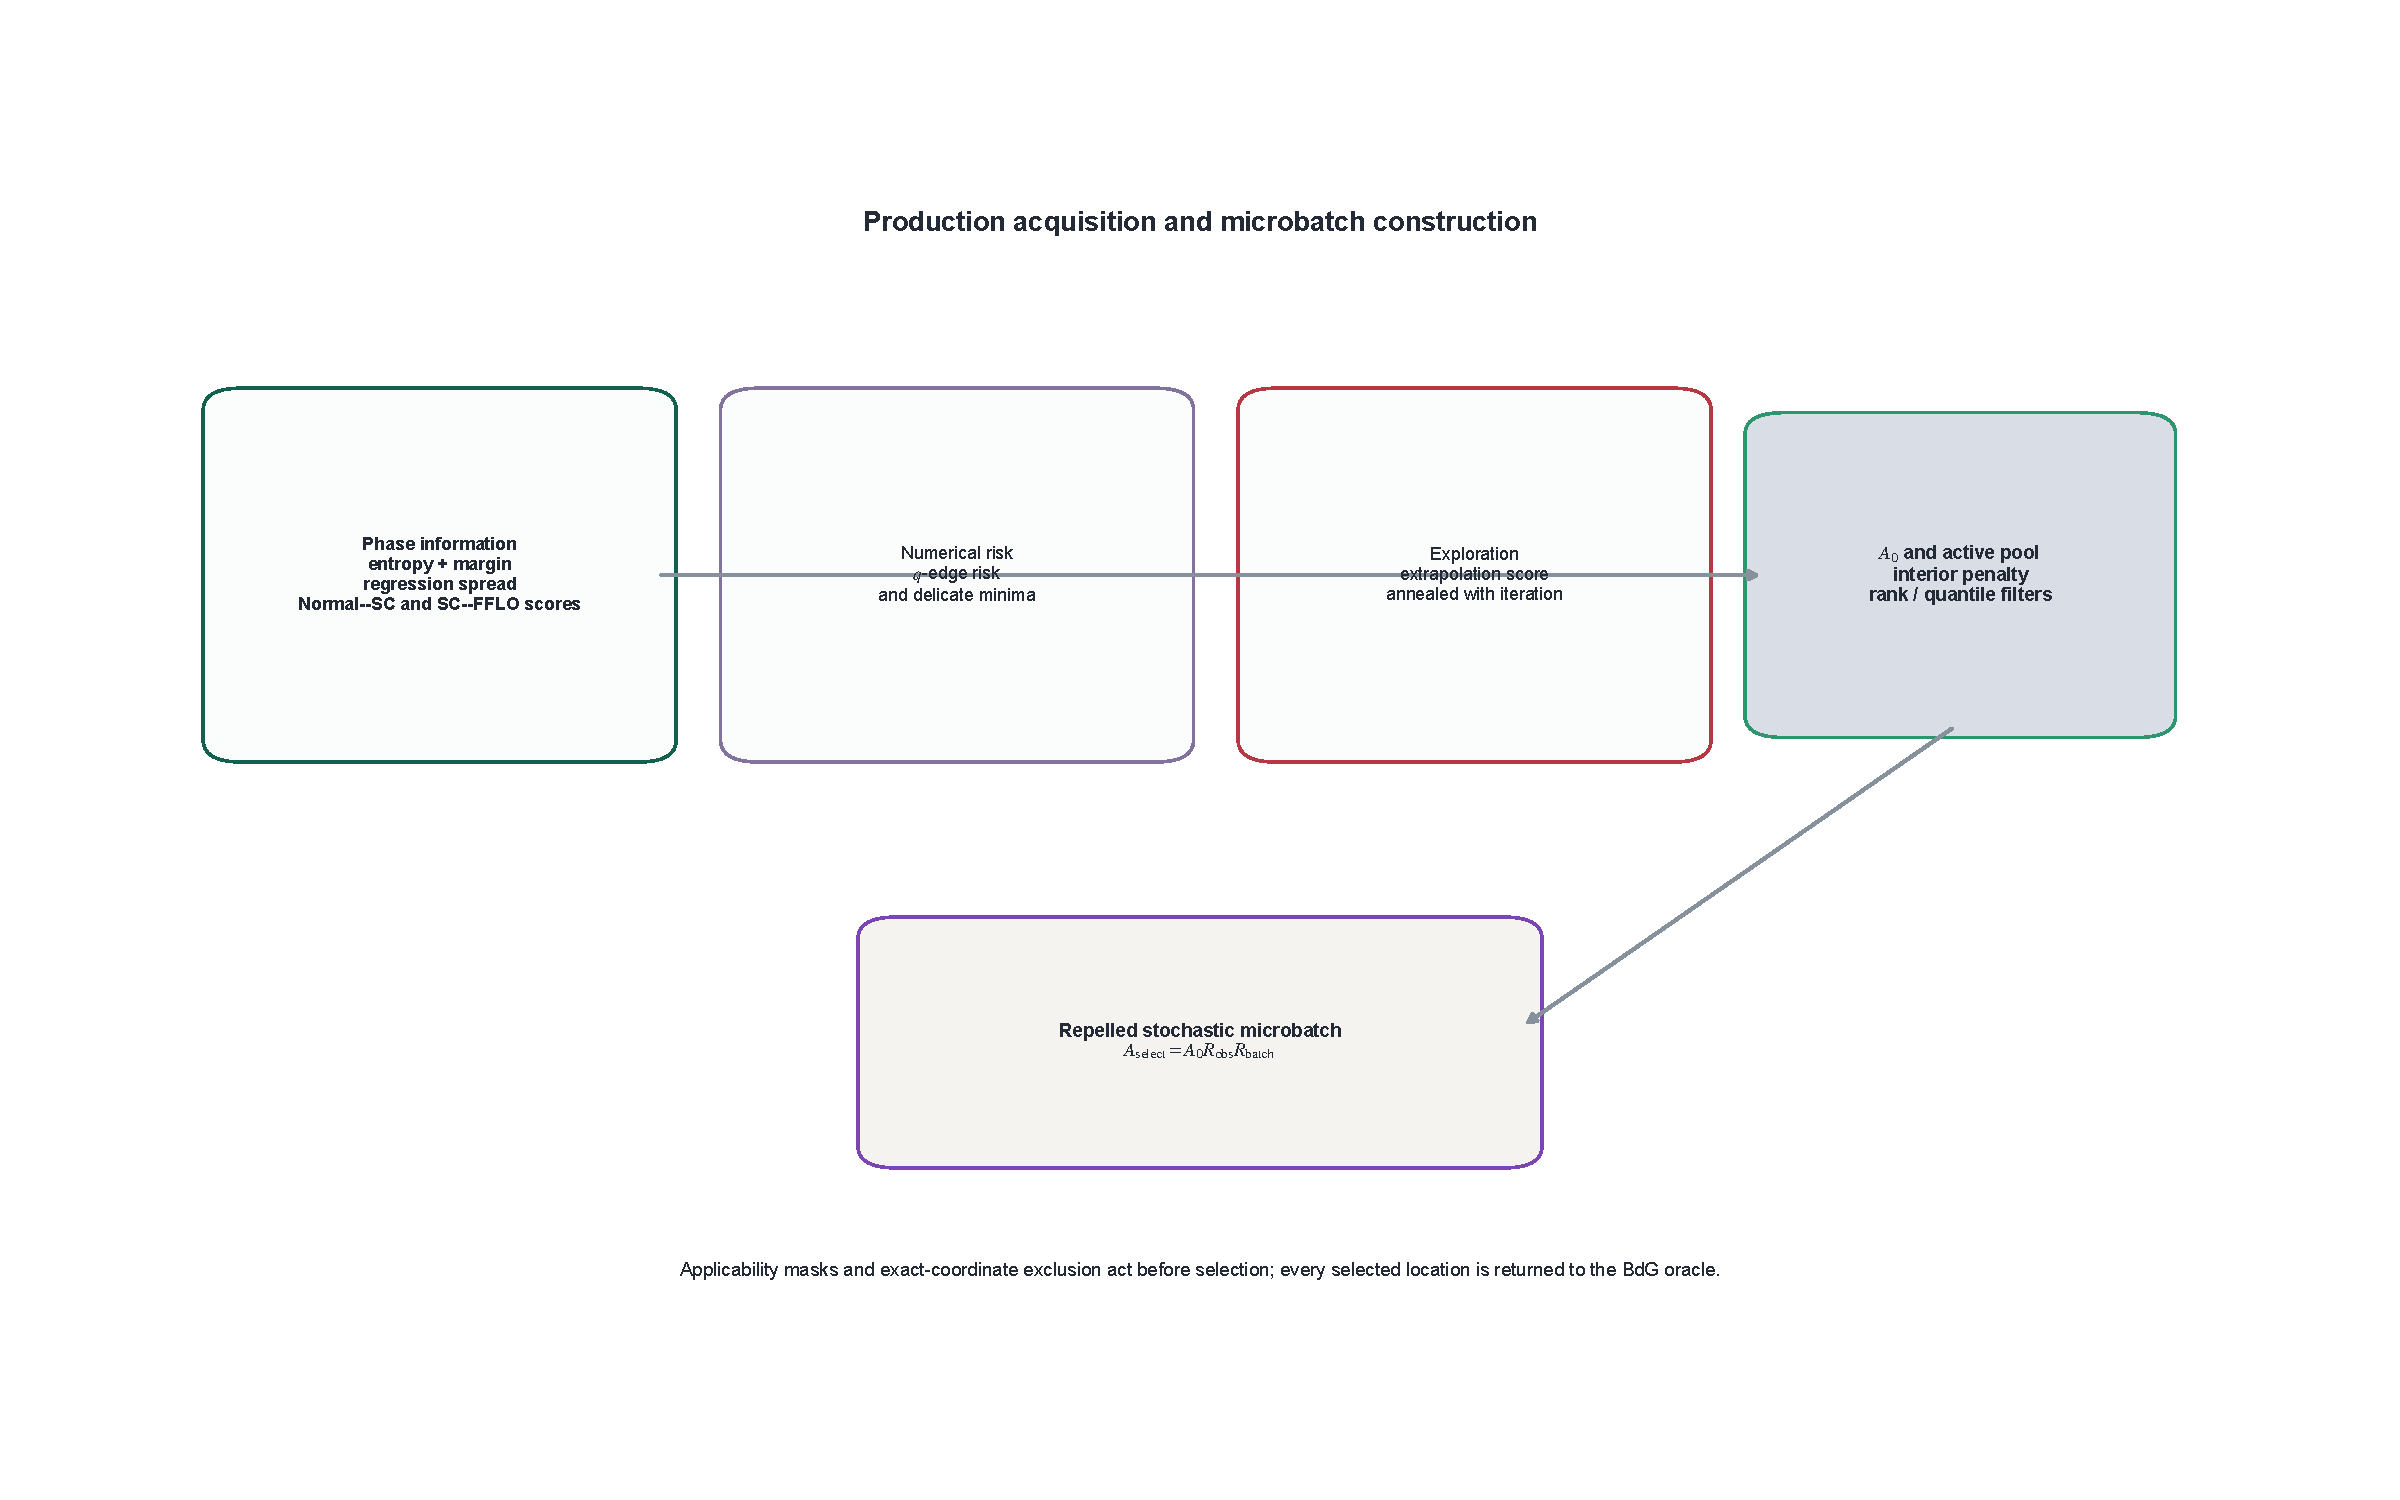
\includegraphics[width=\columnwidth]{figures/S3_acquisition_decomposition.pdf}\caption{Acquisition decomposition and repelled microbatch selection.}\end{figure}

\section{Sampling efficiency}
The Stage-I candidate universe is the complete $241\times321$ Cartesian grid over $k_BT/t\in[0,0.56]$ and $J_A/t\in[0,2.12]$, containing 77,361 locations. The final primary discovery dataset contains 6,880 unique exact coordinates. Thus $f_{\rm exact}=6880/77361=0.08893$ and $R_{\rm call}=77361/6880=11.24$. The archived selection tables contain 8,192 call records and 7,305 unique selected coordinates; these counts differ because returned, accepted, and duplicate-accounting layers are not interchangeable. A boundary-enrichment factor cannot be reconstructed because the export does not retain complete per-iteration candidate-pool boundary labels. Per-iteration wall times exist, but a matched exhaustive-grid baseline does not, so no wall-time speedup is claimed.
\begin{table}[h]\caption{Sampling and exact-call accounting.}\centering\small\begin{tabular}{lr}\toprule Quantity&Value\\\midrule candidate locations&77,361\\ selected call records&8,192\\ unique selected coordinates&7,305\\ unique exact coordinates&6,880\\ training-eligible records&6,880\\ reliable exact records&6,104\\ sampling fraction&8.893\%\\ exact-location reduction&11.244$\times$\\ boundary enrichment&not recoverable\\ wall-time speedup&not established\\\bottomrule\end{tabular}\end{table}
\begin{figure}[h]\centering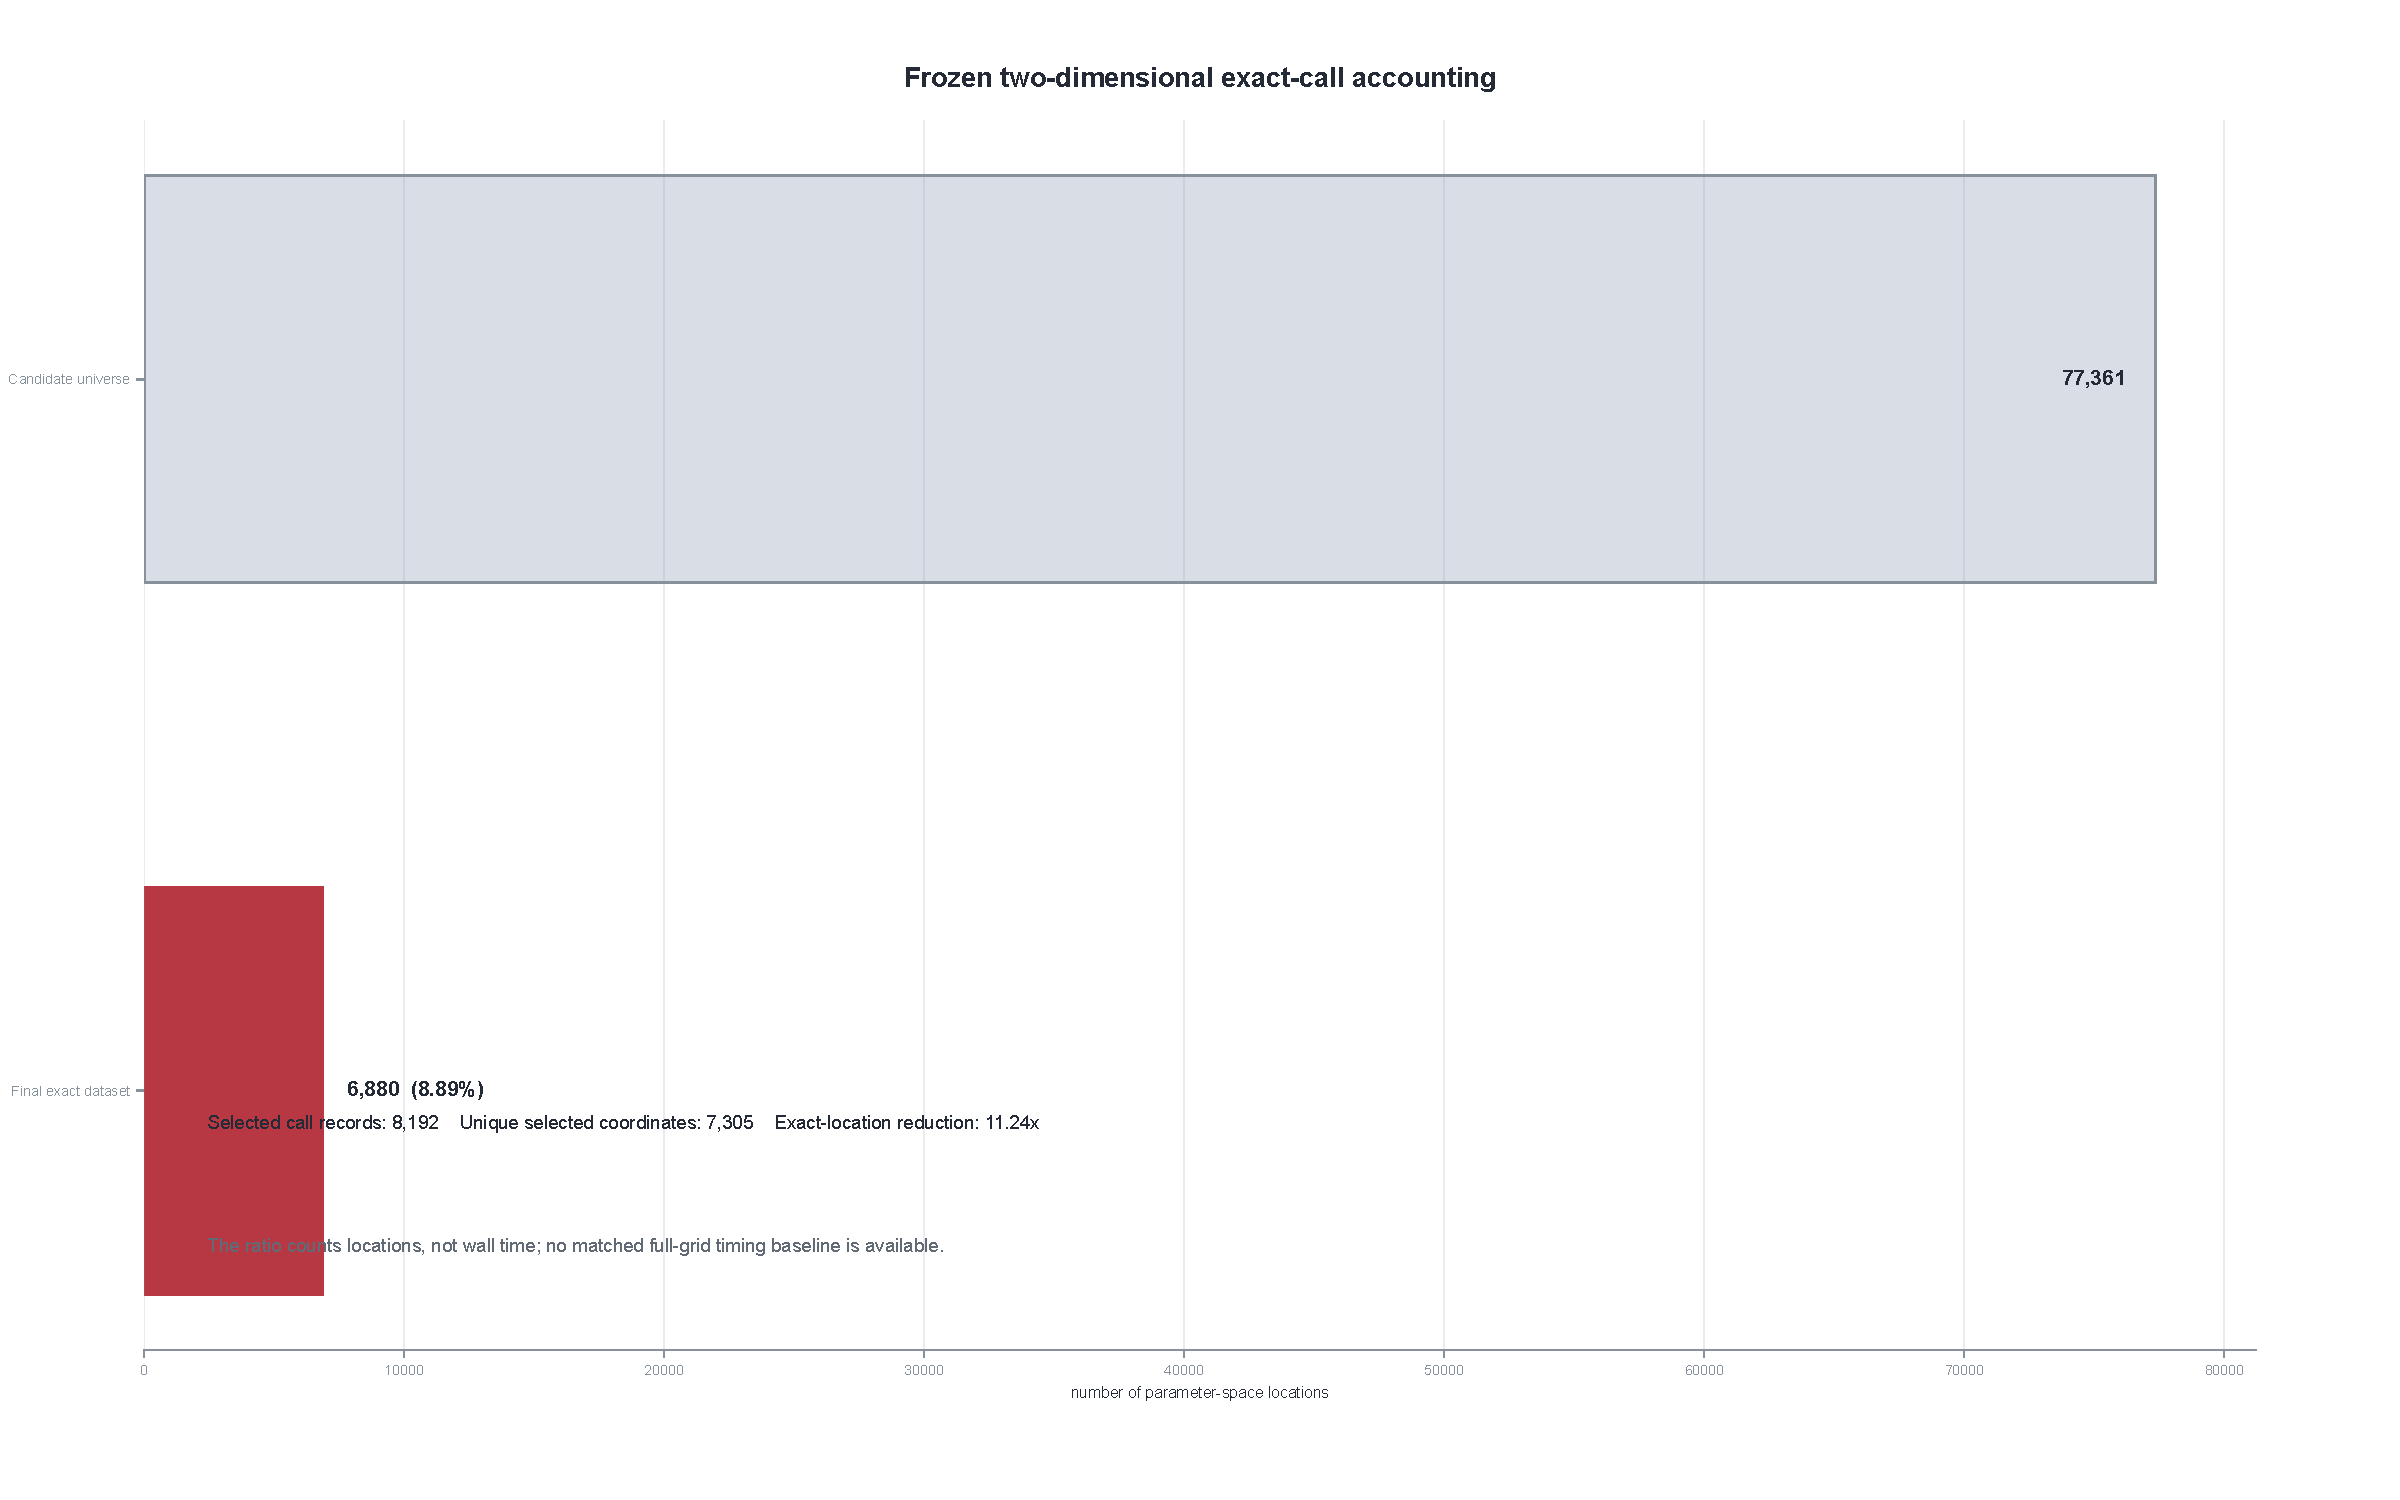
\includegraphics[width=\columnwidth]{figures/S4_sampling_efficiency.pdf}\caption{Frozen candidate-universe and exact-location accounting.  The reduction is a location-count ratio, not a wall-time acceleration.}\end{figure}

\section{Numerical diagnostics and operational stopping}
These criteria are operational controls for the numerical workflow. They are not thermodynamic observables or universal physical scales. Phase-map change is the fraction of fixed monitor-grid cells whose predicted phase changes between iterations. Boundary displacement is a bidirectional nearest-neighbor $p_{95}$ distance between successive extracted boundary point sets after normalization by the parameter-domain ranges. Coverage is the $p_{95}$ distance from the current monitor-grid boundaries to exact samples. Surprise is the fraction of returned labels that differ from the prior prediction, with trusted and flagged denominators stored separately. Four of five main conditions must hold for four successive iterations after a five-iteration minimum. The adopted thresholds reflect the monitor-grid resolution and workflow tolerance, not a physical scale.
\begin{table*}[t]\caption{Operational diagnostics.}\centering\small\resizebox{\textwidth}{!}{\begin{tabular}{lllll}\toprule Diagnostic&Definition&Domain&Operational setting&Interpretation\\\midrule phase-map change&changed-cell fraction&fixed $241\times321$ monitor&$<0.002$&map stability\\ Normal--SC shift&bidirectional $p_{95}$&normalized domain&$<0.004167$&boundary stability\\ SC--FFLO shift&bidirectional $p_{95}$&normalized domain&$<0.004167$&boundary stability\\ coverage&boundary-to-exact $p_{95}$&normalized domain&$<0.00625$&sampling support\\ label surprise&prediction/return mismatch&selected calls&$<0.05$&sequential stability\\ patience&successive eligible iterations&iteration history&4&operational termination\\\bottomrule\end{tabular}}\end{table*}

\section{Topology diagnosis and reconstruction sensitivity}
Topology is applicable only to thermodynamically accepted, numerically reliable, gapped FFLO states.  The minimum absolute BdG eigenvalue is scanned over the full Brillouin zone.  At $k=0,\pi$, the analytic Pfaffians are
\begin{align}P_0&=(\mu-t\cos(q/2))^2+\Delta^2-(\lambda_y\sin(q/2))^2-(J_A\cos(q/2)+\lambda_z\sin(q/2))^2,\\P_\pi&=(\mu+t\cos(q/2))^2+\Delta^2-(\lambda_y\sin(q/2))^2-(J_A\cos(q/2)+\lambda_z\sin(q/2))^2.\end{align}
Away from the relative Pfaffian tolerance $10^{-8}$, $P_0P_\pi<0$ gives $\nu=1$ and $P_0P_\pi>0$ gives $\nu=0$. Analytic values were checked against direct Majorana-basis Pfaffians, and CPU/GPU full-zone gaps were compared in the archived topology validation. The displayed transition contour is a deterministic support-restricted reconstruction on a $401\times401$ monitor grid with support radius 0.045.  For neighborhoods $k=6,8,12$, its arc lengths are 0.8270, 0.8215, and 0.8038, while coverage $p_{95}$ is 0.006269, 0.006185, and 0.005913. This sensitivity and the local opposite-$\mathbb Z_2$ brackets make the contour a guide to the gap-closing region rather than an exact boundary; nodal alternatives are not exhaustively excluded.

\section{Three-dimensional extension}
Stage IV samples $(k_BT/t,J_A/t,\mu/t)$ with $\mu/t\in[-0.5,1.5]$. The main figure shows the exact thermodynamic point cloud, reliable FFLO topology support, and bins centered at $\mu/t=-0.45,0.15,0.85,$ and $1.45$ with half-width 0.025. No interpolation is performed between slices. Archived map-change, proxy-surface displacement, coverage, surprise, and component-count histories are retained as numerical diagnostics only. The discrete support reveals systematic three-dimensional structure but does not establish a converged continuous topology surface or complete atlas.

\section{Reproducibility, code, data, and environment}
{\small The source registry maps exact evaluation, surrogate training, acquisition, stopping, and topology to public modules. Frozen configuration: Python 3.10.20, PyTorch 2.11.0+cu130, seed 42, and eight H100 shards with round-robin partitioning. Archived runs retain configurations, selected coordinates, exact shards, dataset views, checkpoints, monitor predictions, and stop history. Regeneration uses \path{figures/build_publication_supplement_figures.py} and \path{manuscript_langgraph/scripts/run_public_manuscript_reproducible.py}. Because the export lacks Git metadata, SHA-256 hashes identify inputs and outputs.\par}
